%!TEX root = ../thesis.tex
%*************************************************************************************
%*********************************** Methodology chapter *****************************
%*************************************************************************************

%%% Discursive explanation of Value of Information theory
% Make it super approachable/accessible, make sure to give plain explanations of everything and discuss interpretations thoroughly
% Build up the theory with an example problem alongside, starting from simple optimization (very briefly). I.e. every time a new concept is introduced in theory, develop the example problem further to highlight that aspect. Also write a python notebook developing the ideas and numerics (copy over wording where possible). Would be good to include a brief tirade about constraints in probabilistic problems and how strict (failable) constraints don't really make sense. Would be nice to have the example energy systems related, maybe something like a simple solar-battery system sizing problem, initially starting with a very simple model (e.g. limited set of choices, simple sim with no uncertainty), and then building up the complexity (e.g. adding uncertainties \& decision variables to show flexibility of influence diagram, doing optimization in continuous space vs discretization - show runtimes, etc.) until it becomes a full stochastic LP with VoI (could start off with operational LP as simulator to keep things neat, but comment that any simulator would be fine). Could keep it simplistic but of a similar form to the BD-VOI work and then comment on the link to that more complex model version.

%%%
\graphicspath{{Methodology/Figs/}}

% Tikz settings for decision tree diagrams
\tikzset{%
>={Latex[width=3.5mm,length=3.5mm]},
  % Specifications for style of nodes:
  base/.style = {text centered, very thick},
  DTnode/.style = {draw=black, minimum width=1.5cm, minimum height=1.5cm, align=center, font=\sffamily\LARGE, inner sep=5pt},
  triangle/.style = {shape=regular polygon, regular polygon sides=3, inner sep=3pt},
  dummy/.style = {minimum width=2.25cm, minimum height=2.25cm},
  annot/.style = {draw=none, minimum width=0cm, minimum height=0cm, align=center, font=\sffamily\normalsize}
}
\newcommand{\tkzhsep}{3.5cm}
\newcommand{\tkzlabsep}{1.1cm}
\newcommand{\tkznodeysep}{1cm}
%%%


\chapter{\glsxtrlong{voi} analysis} \label{chap:methodology}

\begin{cbox}{}
    This chapter ...\\

    \printpublication{langtry2025todo}

\end{cbox}

\newpage

% Brief intro to chapter explaining contents and flow.
\noindent
\glsxtrlong{voi} analysis (\glsxtrshort{voi}) is the main methodology used in this thesis to investigate the benefit of data collection for improving decision making. This chapter explains the \glsxtrlong{voi} framework. It begins with a brief introduction to \glsxtrshort{voi} and its history in \Cref{sec:methodology-intro}. The theory of the framework is then progressively built up through Sections \ref{sec:methodology-statistical-decision-theory} to \ref{sec:methodology-framework-extensions}. Alongside this theory, the interpretation of what the calculations are doing and their meaning is discussed, and a worked example of a simple building energy system is developed to illustrate how the results can inform decision making. Finally, the limitations of the framework are explored in Section \ref{sec:methodology-limitations}. % and practical considerations for computing \glsxtrshort{voi} values ... and \ref{sec:methodology-considerations}.

%********************************** VoI intro section **************************************
\section{Introduction} \label{sec:methodology-intro}

% Nab from group VoI intro and other papers
% Explain the history of VoI, what it does (i.e. the question it answers), and where it has been used in the past (propose that it'd be extremely useful in the insurance industry)

\glsxtrlong{voi} analysis is a numerical framework for quantifying the expected benefit of collecting data to improve decision making by reducing uncertainty. The economic form was originally proposed by \citep{raiffa1961AppliedStatisticalDecision}\footnote{Though several other authors were working on similar ideas in other fields around the same time \citep{howard1966InformationValueTheory,hurley1964MathematicalTheoryValue,spivey1968DecisionMakingProbabilistic,feltham1968ValueInformation,szaniawski1967ValuePerfectInformation}}, and is built on Bayesian Decision Analysis and Expected Utility Theory \citep{smith1945TheoryGamesEconomic}. It investigates how reducing epistemic uncertainty in a system (uncertainty associated with a lack of knowledge of a system \citep{zhang2021ValueInformationAnalysis}) by taking measurements affects the average utility/performance of the decisions within that system. It numerically answers the question,

\begin{cbox}[colback=Aquamarine!10!white]{}
How much better on average would a decision maker do at a given problem by taking a measurement to reduce uncertainty before making their decision?
\end{cbox}\

\noindent
This question has been and remains extremely important in lots of disciplines, and \glsxtrshort{voi} has been used to study it in a wide variety of contexts. Early applications in the 1970s included \citep{conrad1980QuasiOptionValueExpected}, operations management \citep{bedford1966MeasuringValueInformation}, agriculture \citep{perrin1976ValueInformationValue}, accountancy \citep{mock1971ConceptsInformationValue}, wargaming \citep{oldham1996ValueInformation}, and hydrology \citep{klemes1977ValueInformationReservoir}. Due to the limited computational power available at the time, these studies used simple decision tree models of uncertainties and decision making. However, due to the interest in linear \glsxtrlong{sp} in Operations Research and Management Science at the time \citep{williams1965StochasticLinearProgramming,dantzig1955LinearProgrammingUncertainty,wilson1966ProgrammingUncertainty} following the success of \glsxtrlong{lp} in supply chain management \citep{dantzig1956RecentAdvancesLinear}, a few studies applied \glsxtrshort{voi} to decision making using small, early Linear Programs \citep{avriel1970ValueInformationStochastic}.

% Note: copied from VoI section of Lit Review
More recent uses include fields such as environmental science, medicine, agriculture, and economics \citep{keisler2014ValueInformationAnalysis}. For example in medicine, \glsxtrshort{voi} has been used to study the trade-off between reducing uncertainty in the efficacy of treatments and the cost of performing clinical trials \citep{willan2005ValueInformationOptimal}, and to decide whether further research is required before a new medical technology is adopted \citep{tuffaha2014ValueInformationAnalysis}.

Within engineering, \glsxtrshort{voi} has been used in contexts such as maintenance scheduling for buildings \citep{grussing2018OptimizedBuildingComponent} and wind farms \citep{myklebust2020ValueInformationAnalysis}, construction project planning \citep{esnaasharyesfahani2020PrioritizingPreprojectPlanning}, automotive design \citep{acar2009SystemReliabilityBased}, sensor placement \citep{malings2016ValueInformationSpatially}, and structural health monitoring \citep{difrancesco2021DecisiontheoreticInspectionPlanning,difrancesco2023SystemEffectsIdentifying}.

Review papers \citep{keisler2014ValueInformationAnalysis} and \citep{zhang2021ValueInformationAnalysis} provide thorough overviews of the applications of \glsxtrshort{voi} across disciplines and in engineering respectively.


%********************************** VoI theory section **************************************
\section{Statistical decision theory} \label{sec:methodology-statistical-decision-theory}

% Build up from the ground starting off with brief explanations of what we mean by optimization, expectations, etc., including notation

To understand how uncertainty affects decision making in a quantifiable way, we first need a mathematical framework for making decisions. For this we'll use the mathematics of optimisation\footnote{In the energy systems field this is referred to as optimisation based design/control \citep{barber2022ReviewOptimizationBased}}. Numerical optimisation provides us with a well-defined, objective, and consistent way to make decisions, which does not rely on unquantifiable human judgement\footnote{Of course the setup of our optimisation \textit{is} determined by subjective human judgement. We need to define what we care about, i.e. what objective we want to optimise and what our constraints are. We can never really achieve complete objectivity. But, given a particular problem we want to solve, with a goal we can quantify, optimisation give us an objective tool for tackling it.}.\\

Let's imagine we have some problem we want to solve\footnote{We are the decision maker, also called the `actor'.}, and to do so we have to select one choice, which we'll call an `action' $a$, from a set of possible actions, $\mathcal{A}$. How well each action does at our problem is described by a utility function, $u(a)$. Our actions can have multiple aspects (or dimensions), and the utility function returns a single number for each action which describes how `good' it is at solving the problem. % For example, ...
Costs can be described with negative utilities.

We want to find the best action to take, that is the one which achieves the highest utility. Mathematically we describe this optimisation problem\footnote{Mathematics uses somewhat different notation from decision theory to describe optimisation problems, see \citep{boyd2004ConvexOptimization}.} as,
\begin{equation}
    \mathlarger{\max_{a \in \mathcal{A}} \: u(a)}
\end{equation}
How to actually search through the set of possible actions to find the optimal choice for a practical problem is a complicated question. There are many \textit{many} different optimisation algorithms, all of which are suited to different situations \citep{bonnans2006NumericalOptimizationTheoretical}. But for our purposes, let's assume we can choose a suitable method for our problem, and that we are able to properly optimise our utility to find the best action, which is the one we'll take.\\

This is a simple deterministic model of decision making which assumes we know exactly how the action we take will perform. However in practical engineering systems, there are usually factors which we don't precisely know at the time the decision is made that affect how the different actions will perform when taken, i.e. the utility they achieve. Because of these uncertain factors, which we'll refer to as the `uncertainties' of the system, $\theta$, there are many possible outcomes if a given action is taken. We can graphically represent this process of taking an action, realising the value of the uncertainties, and observing an outcome/utility, using a decision tree which is illustrated in \Cref{fig:methodology-DT-prior}.

\begin{figure}[h]
    \vspace*{-1.5cm}
    {\centering
    \begin{tikzpicture}[node distance=0cm]

    % Nodes
    \node[DTnode, rectangle] (action) at (0,0) {$A$};
    \node[annot, below of=action, yshift=-\tkzlabsep] {$a \in \mathcal{A}$};
    \node[DTnode, circle, right of=action, xshift=\tkzhsep, yshift=\tkznodeysep] (theta) {$\theta$};
    \node[annot, below of=theta, yshift=-\tkzlabsep] {$\theta \sim \pi(\theta)$};
    \node[DTnode, triangle, right of=theta, xshift=\tkzhsep, yshift=-\tkznodeysep] (utility) {$U$};
    \node[annot, below of=utility, yshift=-\tkzlabsep] {$u\left(a,\theta\right)$};

    % True arcs
    \begin{scope}[ultra thick]
        \draw[->] (action) -- (theta);
        \draw[->, dashed] (theta) -- (utility);
    \end{scope}

    % Dummy nodes
    \node[DTnode, dummy, circle, draw=none, below of=theta, yshift=2*\tkznodeysep]  (dt1) {};
    \node[DTnode, dummy, circle, draw=none, below of=theta, yshift=-2*\tkznodeysep]  (dt2) {};
    \node[DTnode, dummy, circle, draw=none, below of=theta, yshift=-4*\tkznodeysep]  (dt3) {};

    \node[DTnode, dummy, circle, draw=none, below of=utility, yshift=4*\tkznodeysep]  (du1) {};
    \node[DTnode, dummy, circle, draw=none, below of=utility, yshift=2*\tkznodeysep]  (du2) {};
    \node[DTnode, dummy, circle, draw=none, below of=utility, yshift=-2*\tkznodeysep]  (du3) {};

    % Dummy arcs
    \begin{scope}[draw=gray]
        \draw[-] (action) -- (dt1);
        \draw[-] (action) -- (dt2);
        \draw[-] (action) -- (dt3);
        \draw[-] (theta) -- (du1);
        \draw[-] (theta) -- (du2);
        \draw[-] (theta) -- (du3);
    \end{scope}

    \end{tikzpicture}
    \vspace*{-1.5cm}
    \caption{Decision tree representation of decision making under uncertainty.} \label{fig:methodology-DT-prior}
    \vspace*{0.15cm}
    {\hfill
    \footnotesize{Adapted from Figure 1 of \citep{difrancesco2021DecisiontheoreticInspectionPlanning}}
    \hfill}
    }
\end{figure}

While we don't know the value of the uncertainties, and so the outcome that we'll get, we typically do have probabilistic knowledge of them. This knowledge comes in the form of their probabilistic model or distribution\footnote{In this chapter will assume that you are somewhat familiar with probabilities, likelihoods, sampling from distributions, and calculating expectations. If not, there are many textbooks and courses that introduce these statistical ideas, such as \citep{schwarzlander2011ProbabilityConceptsTheory}.}\fnsep\footnote{The distributions of the uncertainties can either be modelled using existing data from similar system, or by making reasonable assumptions based off knowledge of the system. The choice of these distributions is a critical modelling step \citep{vandeschoot2021BayesianStatisticsModelling}.}, $\pi(\theta)$.

As the utility now depends on both the action and the value of the uncertainties, $u(a,\theta)$, there is now also uncertainty or risk associated with the utility we'll get, which we must manage during decision making. There are many ways of handling this risk, such as taking the action with the `best worst-case' utility, or the one with the best robustness guarantees. But the most common way is to take the action with the highest average (or expected) utility\footnote{The framework can be easily adapted to use whichever uncertainty management method is most appropriate for the decision making context. This is done by simply changing the objective. For example in \Cref{chap:parks}, a \glsxtrlong{cvar} term is added to the objective to incorporate risk aversion into the decision making. In fact, many risk management methods just adjust the utility function, adding a risk term, and still optimise the expectation.}. So the `objective' we now want to optimise to determine our action choice is the expected value of the utility over the uncertainties in the system,
\begin{equation} \label{eq:methodology-prior-optimisation}
    \mathlarger{\max_{a \in \mathcal{A}} \: \mathbb{E}_{\theta}\lbrace u(a,\theta) \rbrace}
\end{equation}\\

\noindent
However, for real engineering problems we typically cannot calculate this expectation exactly\footnote{The expectation can only be calculated exactly if the probabilistic model of the uncertainties used is discrete, or if the utility function is very simple.}. Instead, we use a \glsxtrlong{mc} (\glsxtrshort{mc}) estimate to approximate it\footnote{In this thesis, whenever there is an expectation, we will use an \glsxtrshort{mc} estimate of it in our numerical calculations.}. To do so, we draw a number of samples from the distributions of the uncertainties, $\theta^{(n)} \sim \pi(\theta)$, and compute the average utility over those samples,
\begin{equation}
    \mathlarger{\frac{1}{N} \sum_n u\big(a,\theta^{(n)}\big)}
\end{equation}
As the number of samples used, $N$, increases, this approximation improves, and the estimate converges to the true value of the expectation.

So to solve our decision making problem under uncertainty, we optimise the average utility achieved over the sampled values of the uncertainties,
\begin{equation}
    \mathlarger{\max_{a \in \mathcal{A}} \: \mathbb{E}_{\theta}\lbrace u(a,\theta) \rbrace \: \approx \: \max_{a \in \mathcal{A}} \: \frac{1}{N} \sum_n u\big(a,\theta^{(n)}\big)}
\end{equation}
Doing so tells us the best action to take, $a^*$, and how `good' we expect it to be at solving our problem, i.e. the average utility it achieves. We can also use the distribution of its utility over the uncertainty samples to understand the risk associated with our decision making.\\

More generally, this type of optimisation is referred to as a `stochastic decision problem'. It is fully specified by the set of possible actions, $\mathcal{A}$, the probabilistic model of uncertainties, $\pi(\theta)$, and the utility function\footnote{Strictly, it's the optimisation objective which is a function of the utility that defines the problem, but these are often used interchangeably.}, $u(a,\theta)$. Solving the stochastic optimisation in Eq. \ref{eq:methodology-prior-optimisation} gives us the best solution to this problem. But solving it can be very computationally expensive, as the utility function needs to be evaluated $N$ times due to the sampling\footnote{In fact for a Stochastic Program, the computational cost of using this average utility scales as $\mathcal{O}(N^3)$.}. Instead, we could try to solve the problem using some heuristic \citep{pickering2016ComparisonMetaheuristicLinear}. A common approach is to use the expected (average) values of the uncertainties in a deterministic optimisation, which is called the \glsxtrlong{evp} (\glsxtrshort{evp}). This is a much cheaper problem to solve, but may not correctly identify the best action to take. The difference in expected utilities achieved by the stochastic optimisation (Eq. \ref{eq:methodology-prior-optimisation}) and the solution to the \glsxtrshort{evp} tells us how much better we can do at solving the decision problem by accounting for the uncertainties in the system in our optimisation, and is referred to as the \glsxtrlong{vss} (\glsxtrshort{vss}) \citep{bistline2015ElectricSectorCapacity}. Actually, we could use whatever policy we like to try to solve the decision problem. This more general setting is discussed in \Cref{sec:methodology-on-policy-voi}.\\

\begin{ebox}[label=ebox:opt]{Introducing an example problem}
    To help clarify this discussion of mathematics and understand why it's useful to us, let's apply it to something concrete and introduce an example problem. We'll developed this example problem throughout the chapter, and demonstrate how we can use each step of the mathematical framework as we introduce it. Code for all the calculations in this example is available for you to try out and explore at \url{https://github.com/mal84emma/VoI-Tutorial}.

    \subsubsection*{Designing a solar-battery system for a commercial building}
    Let's imagine we want to decarbonise the energy use of a hypothetical commercial building. To do this we plan to install solar panels and battery storage in the building. This equipment is expensive, but by generating our own energy and doing some energy trading with the grid we can reduce the electricity bill. So our goal is to design the solar-battery system for the building, that is choose the sizing of solar panels and battery storage, to minimise the total cost of meeting the building's energy demands.

    To help make this design decision we'll use a simple model of the building energy system to calculate the overall cost of constructing and operating the system, which is described in Appendix \ref{app:example-problem-formulation}.\\

    Initially, we'll optimise the system design by looking at 5 design options selected using our experience of building energy systems, and run the energy model to identify the design with the lowest cost. These design options are chosen to generate between 67\% and 100\% of the building's annual energy demand with the solar panels, and to use between a 4hr and 8hr battery to capture and shift the solar peak. The cost of each design is determined by running the model simulation using data from a single design year, in this case 2017.\\
    % \footnote{The solar capacity factor in Cambridge is roughly 0.13, meaning generating the energy demand over the year (which is 100kW on average) requires roughly 750kW of solar panels.}

    {\centering
    \renewcommand{\arraystretch}{0.8}
    \begin{tabularx}{0.975\linewidth}{ccccc}
        \toprule \toprule
        \makecell{Solar capacity\\(kWp)} & \makecell{Battery capacity\\(kWh)} & \makecell{Capital cost\\(£k/yr)} & \makecell{Operating cost\\(£k/yr)} & \makecell{Annualised\\cost (£k/yr)} \\
        \midrule \midrule
        \multicolumn{5}{>{\centering\arraybackslash}l}{\small\it Discrete design options} \\
        500 & 400 & 65.5 & 100.6 & 166.1 \\
        500 & 600 & 79.5 & 91.4 & 170.9 \\
        600 & 600 & 87.0 & 76.1 & 163.1 \\
        \textbf{750} & \textbf{600} & 98.2 & 54.1 & \textbf{152.3} \\
        750 & 800 & 112.2 & 46.3 & 158.6 \\
        \midrule
        \multicolumn{5}{>{\centering\arraybackslash}l}{\small\it Linear Program solution} \\
        889 & 501 & 101.7 & 39.3 & 141.0 \\
        \bottomrule \bottomrule
    \end{tabularx}
    \bigskip
    \captionof{table}{Deterministic design optimisation results.} \label{tab:example-det-optimisation-results}
    }\

    The results show us that there is a trade-off between the capital and operating costs, and that the design with 750kW of solar panels and 600kWh of battery storage gives us the best balance. With this design, it costs us £152.3k/yr to supply the building load, equivalent to £0.174/kWh. If the solar-battery system wasn't installed, buying all the electricity from the grid would cost £219.2k/yr (or £0.250/kWh), so we save £66.9k/yr (a 31\% cost reduction) by installing the system, as well as significantly reducing our carbon emissions.

    We have in some sense optimised this system design, but we've only looked through a very small number of options. We search through lots more options, but this would be very computationally expensive. However, our building energy system model actually uses a Linear Program to optimise the operation of the system and find lowest cost of running it. So, we can include the solar and battery capacities in our \glsxtrshort{lp} optimisation, and use the nice mathematics of our model to find the actual best capacities and optimal design. This solution is also shown in \Cref{tab:example-det-optimisation-results}. Using the  \glsxtrshort{lp} leads us to a design we might not have chosen to explore. It generates more solar energy than the building can use, and is more cautious with the batteries than we were. And importantly, it reduces the cost by 7.4\% compared to our best design guess.\\

    \newpage
    This design optimisation is all well and good, but we've completely neglected the fact that there are many factors that will affect the operation, and so cost of running of our energy system, that we don't know at the time we design it. So let's introduce some uncertainties into our model, and see how they affect our design decisions. We'll account for uncertainties in the building load, solar generation, and the cost and efficiency of the battery storage. The probabilistic models we'll use are described in Appendix \ref{app:example-problem-uncertainties}.

    We can repeat the optimisations from before, but now we will draw 50 samples\footnote{This isn't that many samples, and so our estimate of the expected cost might have some noisy/inaccurate, but this is the largest number we can use within an achievable computational cost.} from the distributions of the uncertainties, and our design objective will be the average cost from the energy model over these samples. We call a set of values sampled from the uncertainties a `scenario'.\\

    {\centering
    \renewcommand{\arraystretch}{0.8}
    \begin{tabularx}{0.975\linewidth}{ccccc}
        \toprule \toprule
        \makecell{Solar capacity\\(kWp)} & \makecell{Battery capacity\\(kWh)} & \makecell{Av. capital\\cost (£k/yr)} & \makecell{Av. operating\\cost (£k/yr)} & \makecell{Av. annualised\\cost (£k/yr)} \\
        \midrule \midrule
        \multicolumn{5}{>{\centering\arraybackslash}l}{\small\it Discrete design options} \\
        500 & 400 & 65.5 & 95.7 & 161.2 \\
        500 & 600 & 79.6 & 86.4 & 166.0 \\
        600 & 600 & 87.1 & 71.1 & 158.1 \\
        \textbf{750} & \textbf{600} & 98.3 & 49.1 & \textbf{147.4} \\
        750 & 800 & 112.3 & 41.2 & 153.6 \\
        \midrule
        \multicolumn{5}{>{\centering\arraybackslash}l}{\small\it Stochastic Program solution} \\
        807 & 429 & 90.5 & 49.4 & 139.9 \\
        \bottomrule \bottomrule
    \end{tabularx}
    \bigskip
    \captionof{table}{Stochastic design optimisation results.} \label{tab:example-stoch-optimisation-results}
    }\

    Comparing to the results from \Cref{tab:example-det-optimisation-results}, we can see that the same design option is selected as before, but that there is a about a 3\% difference in the estimated cost of the system.
    Designing using the \glsxtrshort{lp}, which is now a Stochastic Program (linear scenario program), leads to a design which uses around 10\% smaller capacities than the deterministic case, but doesn't cause a significant change in total cost between the designs\footnote{Unfortunately we cannot actually compute the \glsxtrshort{vss} as the deterministic LP solution is infeasible, which is a problem, but we can approximate it. This issue is discussed further in Appendix \ref{app:methodology-constraints-tirade}.}.
    So in this case, accounting for these pretty significant uncertainties in our optimisation model doesn't have a substantial impact on the design decision\footnote{Though this might depend on the design year we chose. We may have just got lucky.}, but it does provide us with a better estimate of how much the system might cost\footnote{Not only is the average cost value more accurate, but the statistical information about the possible costs is also useful for planning.}.
\end{ebox}

\newpage
\section{Bayesian decision analysis} \label{sec:methodology-bayesian-decision-analysis}

% Explain what the inclusion of measurements does, how Bayes is applied, and how the framework operates - we now give the decision maker the option to collect data before taking a decision action, which will inform them about the uncertainties and improve their decision making ability

While we are able to manage uncertainties during our decision making, their presence is problematic for decision making. This is because when we are hedging our decision to perform well on average, we're missing out on making the decision that is best for the state of the system (values of the uncertainties) that we actually get. Though of course at the time we are making our decision we don't know what that will be. But, if we were able to reduce the uncertainty in our problem\footnote{Not all uncertainties can be reduced. There are two types of uncertainty. Aleatoric uncertainty, which is inherent variability which cannot be explained away, and epistemic uncertainty, which is uncertainty associated with a lack of knowledge of the system, which can be reduced through data collection. Often in engineering systems uncertain parameters have a mix of aleatoric and epistemic, meaning their uncertainty can be reduced but never fully removed.\label{fn:aleatoric}}, and get better information about the true state of the system, we would need to hedge less and so do a better job of making our decision.

Let's consider how our decision making will change if we are able to take a measurement/collect data that reduces the uncertainties before we have to make our decision.\\

First of all we need to be able to describe how the data informs us of the true state of the system and reduces the uncertainties. We do this using a likelihood function. For a measurement, $e$, the likelihood function, $f_e(z|\theta)$, describes the chance of getting a particular value/data from the measurement, $z$, if the true value of the uncertainties is $\theta$. This is to say it describes the uncertainty associated with the measurement\footnote{A standard likelihood function is a Normal/Gaussian with a precision/variance that is determined from lab experiments, e.g. $\pm10\%$ meaning the standard deviation would be 5\% of the mean (for a 95\% confidence level).}.

Bayes' theorem tells us the following,
\begin{equation}
    p(\theta \mid z) = \frac{p(z \mid \theta) \: p(\theta)}{p(z)} \propto p(z \mid \theta) \: p(\theta)
\end{equation}
where $p(\theta)$ is the prior distribution of the uncertainties, $p(z \mid \theta)$ is the likelihood function of the measurement, and $p(\theta \mid z)$ is the posterior distribution of the uncertainties for a given measurement value/data $z$.

The prior distribution describes our initial knowledge of the uncertainties. The likelihood function describes the knowledge/information we gain from the data. And the posterior distribution combines these two pieces of information, and tells us about the remaining uncertainty given what we've observed. \ph{improve this?}\\

Though the framework is typically described in terms of physical measurements, we can apply these ideas to any source of information that reduces the uncertainty in our problem, such as research, improved forecasting methods, or getting expert advice. The only requirement is that we can model the uncertainty reduction that information provides\footnote{Though if modelling this uncertainty reduction is tricky, we can make a best guess and use sensitivity analysis to see if that guess affects our conclusions.}, i.e. come up with a likelihood function.

As the \glsxtrshort{voi} framework is numerical, we can use a probabilistic programming language such as \href{https://mc-stan.org/}{\texttt{Stan}} \citep{carpenter2017StanProbabilisticProgramming} to sample from the required distributions, giving lots of flexibility in how we can model the uncertainties and how they are reduced by data collection.\\

At the time we're considering whether to take a measurement to support our decision making, we can't know what value/data, $z$, we'll get from the measurement. This means there are many possible outcomes for each available measurement option. Once we've received the data from our measurement, we can use it to form a posterior distribution of the uncertainties, $\pi(\theta|z)$, which has reduced uncertainty compared to the initial, prior distribution. We use this improved information to support and improve our decision making, performing the same stochastic decision process as before, but now using the updated knowledge of the possible outcomes of our actions. We can represent this extra measurement step in the decision making process by extending the decision tree, as shown in \Cref{fig:methodology-DT-prepost}.

\begin{figure}[h]
    \vspace*{-1.5cm}
    {\centering
    \begin{tikzpicture}[node distance=0cm]
    
    % Nodes
    \node[DTnode, rectangle] (measure) at (0,0) {$E$};
    \node[annot, below of=measure, yshift=-\tkzlabsep] {$e \in E$};
    \node[DTnode, circle, right of=measure, xshift=\tkzhsep, yshift=\tkznodeysep] (z) {$Z$};
    \node[annot, below of=z, yshift=-\tkzlabsep] {$z \sim \pi(z)$};
    \node[DTnode, rectangle, right of=z, xshift=\tkzhsep, yshift=-\tkznodeysep] (action) {$A$};
    \node[annot, below of=action, yshift=-\tkzlabsep] {$a \in \mathcal{A}$};
    \node[DTnode, circle, right of=action, xshift=\tkzhsep, yshift=\tkznodeysep] (theta) {$\theta$};
    \node[annot, below of=theta, yshift=-\tkzlabsep] {$\theta \sim \pi(\theta | z)$};
    \node[DTnode, triangle, right of=theta, xshift=\tkzhsep, yshift=-\tkznodeysep] (utility) {$U$};
    \node[annot, below of=utility, yshift=-\tkzlabsep] {$u\left(a,\theta\right)$};

    % True arcs
    \begin{scope}[ultra thick]
        \draw[->] (measure) -- (z);
        \draw[->, dashed] (z) -- (action);
        \draw[->] (action) -- (theta);
        \draw[->, dashed] (theta) -- (utility);
    \end{scope}
    
    % Dummy nodes
    \node[DTnode, dummy, circle, draw=none, below of=z, yshift=2*\tkznodeysep]  (dz1) {};
    \node[DTnode, dummy, circle, draw=none, below of=z, yshift=-2*\tkznodeysep]  (dz2) {};
    \node[DTnode, dummy, circle, draw=none, below of=z, yshift=-4*\tkznodeysep]  (dz3) {};

    \node[DTnode, dummy, circle, draw=none, below of=action, yshift=4*\tkznodeysep]  (da1) {};
    \node[DTnode, dummy, circle, draw=none, below of=action, yshift=2*\tkznodeysep]  (da2) {};
    \node[DTnode, dummy, circle, draw=none, below of=action, yshift=-2*\tkznodeysep]  (da3) {};

    \node[DTnode, dummy, circle, draw=none, below of=theta, yshift=2*\tkznodeysep]  (dt1) {};
    \node[DTnode, dummy, circle, draw=none, below of=theta, yshift=-2*\tkznodeysep]  (dt2) {};
    \node[DTnode, dummy, circle, draw=none, below of=theta, yshift=-4*\tkznodeysep]  (dt3) {};

    \node[DTnode, dummy, circle, draw=none, below of=utility, yshift=4*\tkznodeysep]  (du1) {};
    \node[DTnode, dummy, circle, draw=none, below of=utility, yshift=2*\tkznodeysep]  (du2) {};
    \node[DTnode, dummy, circle, draw=none, below of=utility, yshift=-2*\tkznodeysep]  (du3) {};
    
    % Dummy arcs
    \begin{scope}[draw=gray]
        \draw[-] (measure) -- (dz1);
        \draw[-] (measure) -- (dz2);
        \draw[-] (measure) -- (dz3);
        
        \draw[-] (z) -- (da1);
        \draw[-] (z) -- (da2);
        \draw[-] (z) -- (da3);

        \draw[-] (action) -- (dt1);
        \draw[-] (action) -- (dt2);
        \draw[-] (action) -- (dt3);

        \draw[-] (theta) -- (du1);
        \draw[-] (theta) -- (du2);
        \draw[-] (theta) -- (du3);
    \end{scope}
    
    \end{tikzpicture}
    \vspace*{-1.5cm}
    \caption{Decision tree representation of decision making with measurements} \label{fig:methodology-DT-prepost}
    \vspace*{0.15cm}
    {\hfill
    \footnotesize{Adapted from Figure 1 of \citep{difrancesco2021DecisiontheoreticInspectionPlanning}}
    \hfill}
    }
\end{figure}\

While these decision trees illustrate the sequence of our decision making, the available choices and their possible outcomes, they are only really useful for illustrating simple toy problems. For complex, real world decision making problems, we use influence diagrams to provide a clear and concise visual description of the structure of the system and decision making. These diagrams show only the causal dependencies between decisions, uncertainties, and outcomes in the system, and allow domain experts to quickly describe decision making in complex engineering systems. They are excellently explained by \citep{difrancesco2023GuidanceUseProbabilistic}.\\
% \footnote{... from computational perspective, uncertainties are sampled, and passed as inputs to simulators for variables, which are then inputs to utility calculation ...}

To understand how collecting this data affects our decision making, we can update our decision optimisation to use this improved information that reduces the uncertainties in the problem,
\begin{equation} \label{eq:methodology-posterior-optimisation}
    \mathlarger{\max_{a \in \mathcal{A}} \: \mathbb{E}_{\vartheta|z}\lbrace u(a,\vartheta) \rbrace}
\end{equation}
This new optimisation (stochastic decision problem) can be used to find the decision we would make if we'd received data $z$. We refer to this as the Posterior decision problem, as we are now finding the action that performs best on average under the remaining uncertainty given by the posterior distribution, $\pi(\theta|z)$\footnote{Note, in Eq. \ref{eq:methodology-posterior-optimisation} we use $\vartheta$ to denote estimates of the true value of the uncertainties which are made after data $z$ is received, to differentiate from the possible true values of the uncertainties $\theta$ that we will later average over.}.\\

However, because we don't know what data $z$ we'll receive before we measure, to understand how well we would do using data to support our decision making, we need to average over the possible values of the measurement data\footnote{We also explicitly average over the possible values of the uncertainties, $\theta$, as the measurement values are associated with the true states of the system. During sampling, we first sample $\theta$ values from the prior, and then sample the corresponding likelihood function to obtain $z$ values.},
\begin{equation} \label{eq:methodology-preposterior-value}
    \mathlarger{ \mathbb{E}_{\theta,z} \left\lbrace \max_{a \in \mathcal{A}} \: \mathbb{E}_{\vartheta|z}\lbrace u(a,\vartheta) \rbrace \right\rbrace}
\end{equation}
This tells us how well we would do on average at solving our decision problem, i.e. the expected utility we'd achieve, if we were to gather data to reduce the uncertainties in the problem before making our decision.

We refer to this as the Pre-Posterior decision problem, as we are averaging over all of the possible Posterior decision problems corresponding to each measurement value $z$. Eq. \ref{eq:methodology-prior-optimisation} from before is referred to as the Prior decision problem, as there our decisions are made with only the information from the prior distribution, $\pi(\theta)$.\\

When solving the Pre-Posterior decision problem numerically, we first hypothesis possible values $z$ we could receive from the measurement by sampling from the prior and likelihood functions. Then, for each sampled $z$ value, we consider what the corresponding Posterior decision problem with reduced uncertainty would be, how we would solve it, and how well we would do. Finally, we average those expected utilities to estimate the overall expected utility over solving the decision problem with the help of data collection.

\begin{equation}
    \mathlarger{
        \frac{1}{N} \mathlarger{\sum}_{z^{(n)} \sim f_e(z|\theta^{(n)})} \max_{a \in \mathcal{A}} \Bigg( \frac{1}{M} \mathlarger{\sum}_{\vartheta^{(m)} \sim \pi(\vartheta|z^{(n)})} u\big(a,\vartheta^{(m)}\big) \Bigg)
    }
\end{equation}
\smallskip

\noindent
This means we now get a distribution of the actions we would take given the possible measured values, and how well we would do at solving our problem in each case.\\

Collecting data to reduce the uncertainty in the problem will improve our decision making ability. This is because the decisions we now make are more tailored to the actual state of the system (which we now know more precisely) and use less hedging. We could always take the decision we would initially have made (i.e. our choice from the prior decision problem), but if we see certain data values we can adjust our decision to take a choice better suited to the likely state of the system. We can demonstrate this improvement from uncertainty reduction mathematically,
\begin{equation} \label{eq:methodology-pdp-inequality}
    \mathbb{E}_{\theta,z} \left\lbrace \max_{a \in \mathcal{A}} \: \mathbb{E}_{\vartheta|z}\lbrace u(a,\vartheta) \rbrace \right\rbrace
    >
    \max_{a \in \mathcal{A}} \: \mathbb{E}_{\theta,z} \left\lbrace \mathbb{E}_{\vartheta|z}\lbrace u(a,\vartheta) \rbrace \right\rbrace
    =
    \max_{a \in \mathcal{A}} \: \mathbb{E}_{\theta} \left\lbrace u(a,\theta) \right\rbrace
\end{equation}
\hspace{1.5em}

In the more general case where we have a set of measurement options, $E$, are available to take, we can also optimise our choice of measurement,
\begin{equation} \label{eq:methodology-preposterior-optimisation}
    \mathlarger{
    \max_{e \in E} \: \mathbb{E}_{\theta,z} \left\lbrace \max_{a \in \mathcal{A}} \: \mathbb{E}_{\vartheta|z}\lbrace u(a,\vartheta) \rbrace \right\rbrace
    }
\end{equation}
\hfill \\

\begin{ebox}[label=ebox:bayes]{Measuring building energy usage}
    % Provide probabilistic models (including example of uncertainty reduction from measurement - discuss both perfect and imperfect measurements, and why perfect is unrealistic) and influence diagram for the example problem (explain what nodes and arrows mean)
    % ? Explain how the decision making process would proceed with the measurement included, and discuss how we optimise over the posterior expectation now (same from this new, updated distribution) - kind of already done this, but contextualise
    % Provide the distribution of designs for each hypothesised measurement value (maybe show the utility dist - perhaps with point colour), leave expected utility for VoI part

    Previously in our example problem, we acknowledged that when we design the solar-battery system, we don't know exactly the amount of energy the building will use during operation. And we accounted for this uncertainty in the building load in our design decision, as well as other uncertainties, finding the design that provides the lowest cost on average.

    Our hypothetical commercial building has a design load of 100kW, and from our experience of previous buildings, we expect that the load during operation will be within $\pm20\%$ of this value. So we modelled this uncertain load using a Normal distribution truncated at 2 standard deviations,
    \begin{equation*}
        \theta_{\text{load}} \sim TN(\mu=100, \sigma=10, a=80, b=120)
    \end{equation*}
    This distribution of the load uncertainty, the prior distribution, describes our initial knowledge of the building load, also called our prior knowledge/belief.\\

    We can reduce this load uncertainty by gathering data from the building. For example by collecting monthly energy usage data from the building's electricity meter. Again from our experience of other buildings, we know that the energy usage of a building in future years is likely to be within $\pm5\%$ of the previous year's usage\footnote{Assuming there are no significant changes to the building, e.g. changes of usage or retrofits. At the time of designing the solar-battery system we do not expect any such changes, as heat pumps have recently been installed to decarbonise the building's heating.}.
    So we can describe the information we'd get from this metering data using the following likelihood function,
    \begin{equation*}
        z_{\text{load}}|\theta_{\text{load}} \sim \mathcal{N}(\mu=\theta_{\text{load}}, \sigma=\varepsilon\,\theta_{\text{load}})
    \end{equation*}
    where $\theta_{\text{load}}$ is the uncertain operational building load, $z_{\text{load}}$ is the previous year's load we get from the metering data and use to estimate future loads, and $\varepsilon=0.025$\footnote{To put our experience of future years' energy usage being within $\pm5\%$ of the previous year's within a $95\%$ confidence interval.}.\\

    The uncertainty reduction that collecting this metering data provides is illustrated in Fig. \ref{fig:methodology-example-load-uncertainty-reduction}, which shows the prior distribution of the building load during operation, an example annual load value (measurement) we might get from the electricity meter, and the corresponding posterior distribution.\\

    {
        \centering
        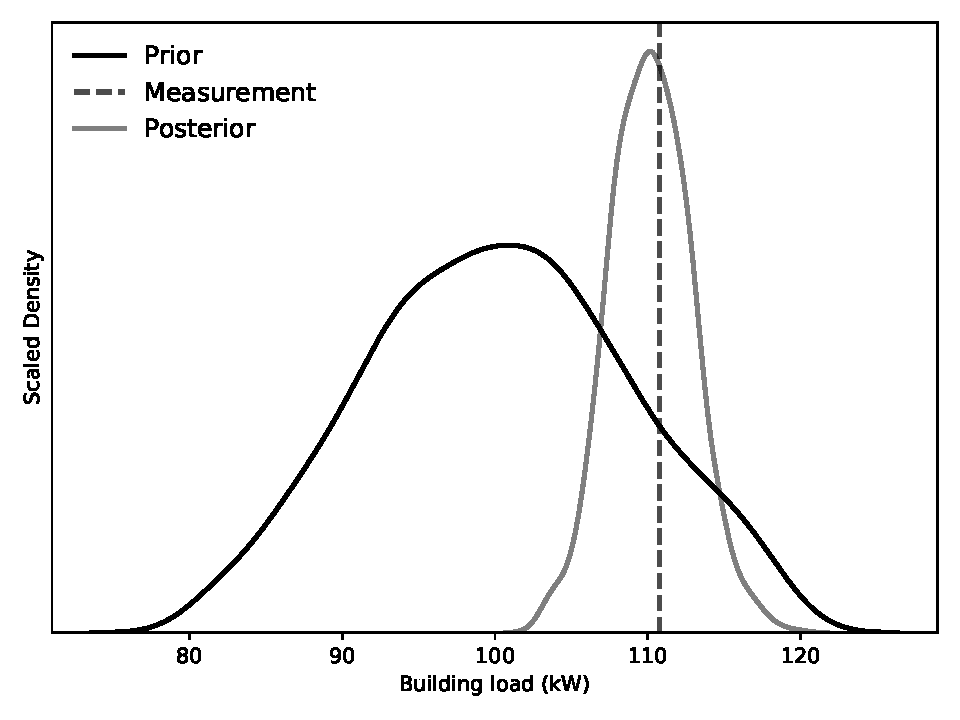
\includegraphics[width=0.66\linewidth]{Methodology/Figs/msr_uncertainty_reduction.pdf}
        \vspace*{-0.25cm}
        \captionof{figure}{Example reduction in load uncertainty provided by metering data.}
        \label{fig:methodology-example-load-uncertainty-reduction}
    }
    \smallskip

    % Think about design decisions with this metering data. Here's the influence diagram ...
    Reducing uncertainty in the building load gives us a better understanding of whether energy we generate with the solar panels can be used by the building, and how much energy we need to store in the batteries to run the building during peak electricity price periods. So, it reduces uncertainty in the operational cost of system designs. This allows us to make a design decision that is better suited to how the building will actually behave.

    We can represent the structure of the solar-battery system design process and how gathering monitoring data affects our decision making using an influence diagram.\\

    {
        \centering
        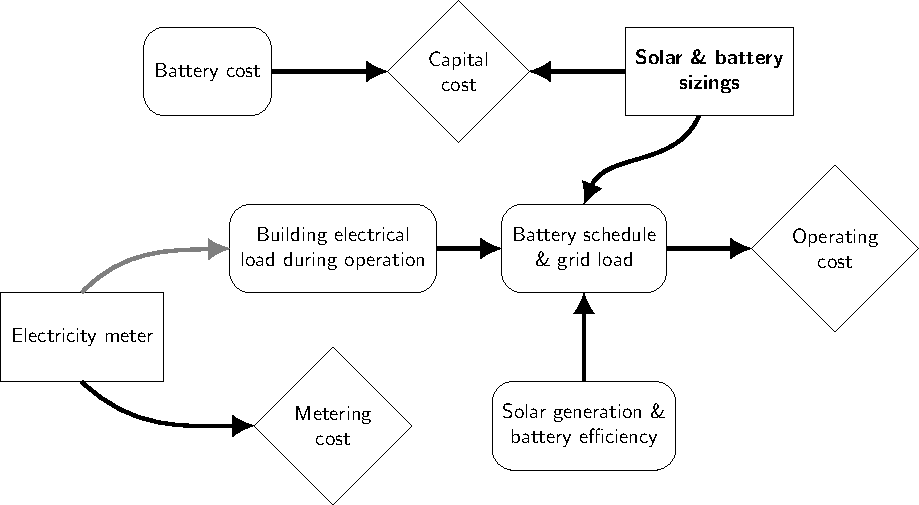
\includegraphics[width=0.75\linewidth]{Influence Diagram/building-design.pdf}
        \vspace*{0cm}
        \captionof{figure}{Influence diagram representation of example energy system design problem.}
        \label{fig:methodology-example-influence-diagram}
        \begin{singlespace}
            \raggedright
            \footnotesize{\it Square nodes represent decisions, rounded nodes represent uncertainties or uncertain factors, and diamond nodes represent outcomes or utilities/costs. Arrows represent causal dependencies between nodes, with grey arrows indicating reduction in uncertainty from data collection.}
        \end{singlespace}
    }
    \hfill\

    To understand how collecting the metering data and reducing load uncertainty might affect our design decision, we can look at the distribution of designs we would choose using our \glsxtrshort{sp} given the possible measurement values we might get. To do so, we hypothesise 50 possible true building load values, $\theta_{\text{load}}$, by drawing from the prior load distribution. We then hypothesise a possible measurement (previous annual load values we get from the metering data, $z_{\text{load}}$) for each true load value by drawing a sample from the corresponding likelihood function\footnote{This is the same as drawing from the joint prior distribution of $\theta$ and $z$.}. The information from each measurement is combined with the prior to form a posterior. And for each measurement value, we perform the design optimisation process by sampling load values from the corresponding posterior, and values for all other uncertainties from their priors as we assume we're not getting information about them, then using the \glsxtrshort{sp} to optimise over these `posterior scenarios' which have reduced load uncertainty.\\

    Fig. \ref{fig:methodology-example-post-designs} shows this distribution of `posterior designs'. Across the designs there is little change in the solar capacity, around $\pm$5\%, however the battery capacity chosen varies by $\pm$25\%. Before, we saw that accounting for uncertainty during the design process didn't have much affect on the chosen design. That is to say that the design that performs best \textit{on average} was similar to the best design for the average scenario\footnote{Specifically, we used the average annual load value in our deterministic optimisation. We're not sure how `average' the year of solar and load profile data we used is. Though there methods for coming up with an `average year' of data, and these are commonly used for energy system design.}.
    However we can clearly see that the uncertainty in building load \textit{does} have a significant effect on the best design for the actual building.\\

    {
        \centering
        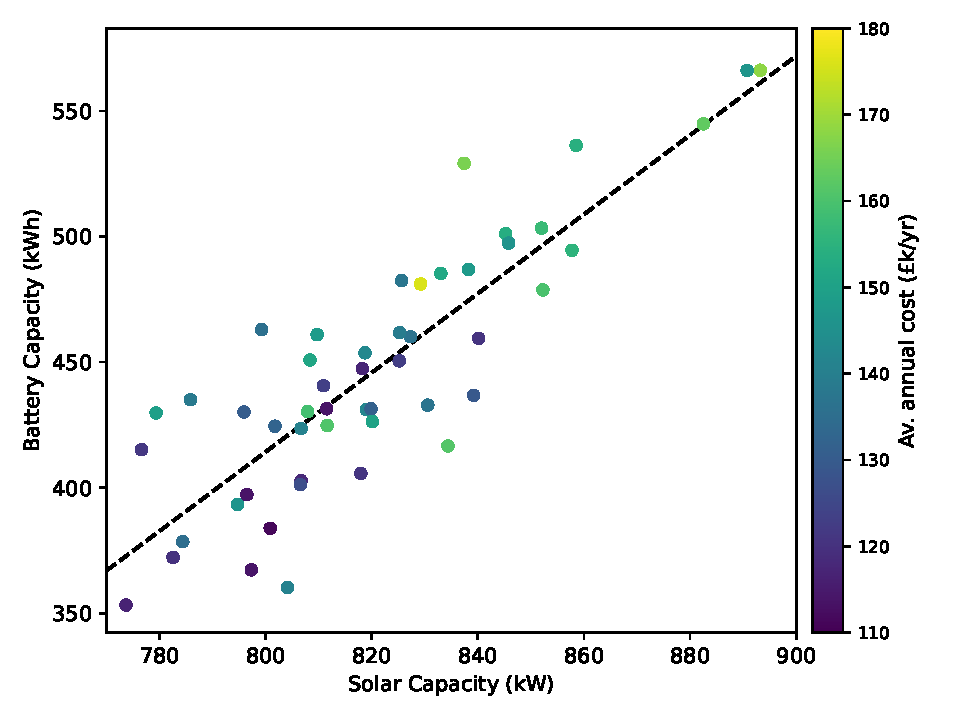
\includegraphics[width=0.75\linewidth]{Methodology/Figs/posterior_designs.pdf}
        \vspace*{-0.25cm}
        \captionof{figure}{Distribution of solar-battery system designs made with metering data.}
        \label{fig:methodology-example-post-designs}
    }
    \bigskip

\end{ebox}

\newpage
\section{The \glsxtrlong{voi}} \label{sec:methodology-voi}

The \glsxtrlong{voi} (\glsxtrshort{voi}) is defined as the difference in the performance of decisions made with and without extra information/uncertainty reduction. So, it is given by the difference between the expected utilities achieved by solving the Prior decision problem (Eq. \ref{eq:methodology-prior-optimisation}) and the Pre-Posterior decision problem (Eq. \ref{eq:methodology-preposterior-value}).
It numerically answers the question,
\begin{cbox}[colback=Aquamarine!10!white]{}
How much better could we do on average if we collected data to reduce the uncertainties in our problem before making a decision?
\end{cbox}
\vspace{0.2cm}

\noindent
If the decision problem has an economic objective (i.e. the utility is a cost or a profit), the \glsxtrshort{voi} tells us how much we should be willing to pay for the data that reduces the uncertainties in our problem. By comparing the \glsxtrshort{voi} to the cost of data collection, \textbf{we can determine if collecting that data is actually worthwhile for supporting our decision making}.\

\subsection{Perfect Information}

Initially let's consider the simplest case of \glsxtrshort{voi}, where we assume we have the ability to perfectly measure the system and remove all uncertainty from our problem. This means the data we collect tells us the true values of the uncertainties, $z=\theta$. So in this case the Pre-Posterior decision problem can be simplified, as the Posterior decision problem is now deterministic, we assume we know the true state of the system we want to optimise for,
\begin{equation}
    \mathlarger{
        \mathbb{E}_{\theta,z} \left\lbrace \max_{a \in \mathcal{A}} \: \mathbb{E}_{\vartheta|z}\lbrace u(a,\vartheta) \rbrace \right\rbrace
        \:\: \rightarrow \:\:
        \mathbb{E}_{\theta} \left\lbrace \max_{a \in \mathcal{A}} \: u(a,\theta) \right\rbrace
    }
\end{equation}
We find the \glsxtrshort{voi} by comparing the average utility achieved by these decisions made with perfect information to the average utility of the Prior decision problem, where the decision is made without any extra information about the uncertainties. In this case the \glsxtrshort{voi} is referred to as the \glsxtrlong{evpi} (\glsxtrshort{evpi}),
\begin{equation} \label{eq:evpi}
    \mathlarger{
        \text{EVPI} =
        \mathbb{E}_{\theta} \left\lbrace \max_{a \in \mathcal{A}} \: u(a,\theta) \right\rbrace
        - \max_{a \in \mathcal{A}} \: \mathbb{E}_{\theta} \left\lbrace u(a,\theta) \right\rbrace
    }
\end{equation}
The \glsxtrshort{evpi} provides an upper bound on all the other \glsxtrshort{voi} values. It is also much cheaper to compute as the posterior optimisations are deterministic. However \glsxtrshort{evpi} values can be misleading, as it's not practically possible to completely remove uncertainty, and so we cannot know how much of that value can actually be obtained.

\begin{ebox}{Value of removing uncertainty}
    Let's imagine what would happen if we were able to perfectly know everything about our building and the solar-battery system we'll put into it, to see how much better we would do if we could achieve the theoretically best possible design. Of course this is unrealistic, some of the uncertainties in the system couldn't be reduced, such as the pattern of solar generation during operation, and for the others we could never completely remove the uncertainty, for example the operational building load couldn't be exactly known. But this thought experiment will give us some insight into how much these uncertainties are affecting our ability to make our design decision.\\

    To do this, we perform a similar process to \ref{ebox:bayes}, but we now sample scenarios from the prior distributions of all the uncertainties, and then use the \glsxtrshort{sp} to find the best design for each scenario, assuming that in each hypothesised case we knew the true values of the uncertainties.

    Fig. \ref{fig:methodology-example-perfect-information} compares the distribution of costs achieved by the initial/prior design (from Table \ref{tab:example-stoch-optimisation-results}) over the scenarios, to the costs of the best possible design for each scenario (the designs made with perfect information).\\

    {
        \centering
        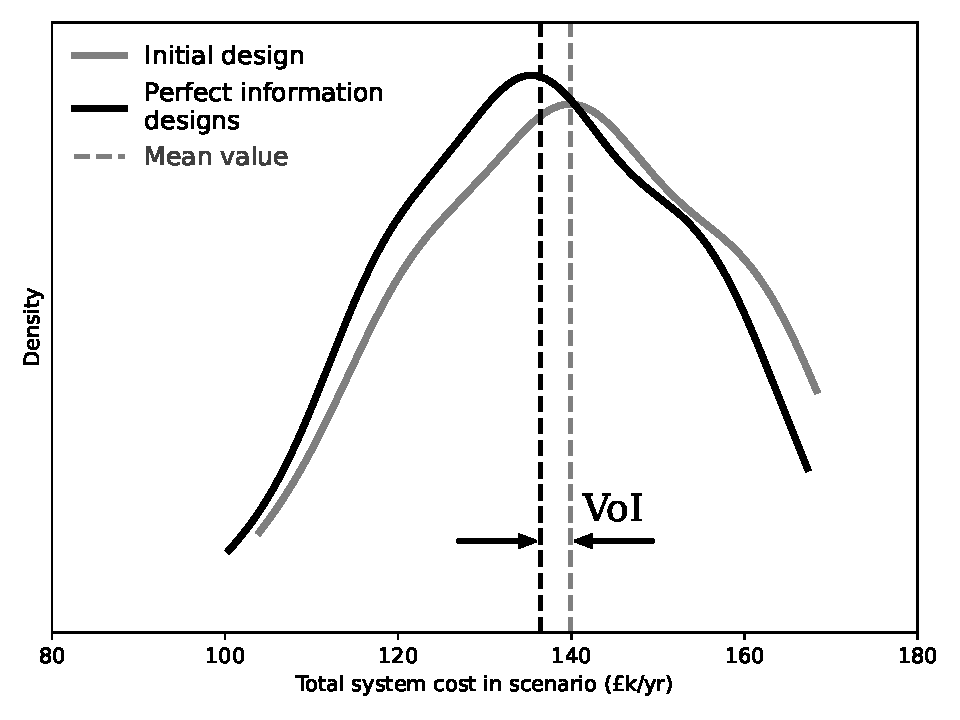
\includegraphics[width=0.75\linewidth]{perfect_info_costs_comparison.pdf}
        \vspace*{-0.25cm}
        \captionof{figure}{Comparing distributions of possible system costs for designs made with and without perfect information.}
        \label{fig:methodology-example-perfect-information}
    }
    \bigskip

    The average cost of the designs made with perfect information is £136.4k/yr. Comparing to the £139.9k/yr average cost of the initial design, the \glsxtrshort{evpi} is £3.5k/yr, or 2.5\% of the prior cost.

    In the context of improving energy system designs to reduce energy costs this is a pretty significant saving. However the \glsxtrshort{evpi} is only an upper bound. So we can't know how much of this cost saving we could actually achieve by collecting data in practice. All we can conclude from this is that reducing the uncertainties in our problem could save us \textit{up to} £3.5k/yr. So it might be worth doing something about the uncertainties to improve our design decision.
\end{ebox}
\vspace{0.1cm}

\subsection{Partial Perfect Information}

Often not all of the uncertainties in a system are, or even can be, reduced (see footnote \ref{fn:aleatoric}). So a more realistic case is one where some uncertainties are removed, but some others remain. This means in the Posterior decision problems, as not all uncertainties are removed, we need to optimise the average utility over the remaining uncertainties. Let's call the uncertainties that are removed by the data collection $\theta$, and the ones that remain unchanged $\phi$. In this case the \glsxtrshort{voi} is referred to as the \glsxtrlong{evppi} (\glsxtrshort{evppi}), and is given by,
\begin{equation} \label{eq:evppi}
    \mathlarger{
        \text{EVPPI} =
        \mathbb{E}_{\theta} \left\lbrace \max_{a \in \mathcal{A}} \mathbb{E}_{\phi} \: \lbrace u(a,\theta,\phi) \rbrace \right\rbrace
        - \max_{a \in \mathcal{A}} \: \mathbb{E}_{\theta,\phi} \left\lbrace u(a,\theta,\phi) \right\rbrace
    }
\end{equation}
\vspace{-0.4cm}

\begin{ebox}[label=ebox:evppi]{Designing with known load}
    If we now only removed the uncertainty in the annual energy usage of the building (or mean load), and so assumed that we knew perfectly at the time of design the aggregate energy demand we'd need to meet, the average cost of our designs made with perfection mean load information would be £139.4k/yr, meaning the \glsxtrshort{evppi} is only £0.5k/yr, or 0.4\% of the prior cost.

    This is a much smaller value than the \glsxtrshort{evpi} we calculated before, which tells us that some of the other uncertainties we're no longer removing have quite a big impact on our design decision. So removing this pretty significant uncertainty ($\pm$20\%) in the mean building load doesn't provide that much of a cost saving for our design. We may decide that it's not worth chasing this saving, and so the upper bound provided by this simplified case can tells us that this information is not worthwhile collecting.
\end{ebox}


\subsection{Imperfect Information}

In the general case, collecting data reduces but does not remove uncertainties\footnote{The previous two perfect information cases are just special cases of this, and provide an upper bound on this general value, \begin{equation*} \mathbb{E}_{\theta,z} \big\lbrace \max_{a \in \mathcal{A}} \: \mathbb{E}_{\vartheta|z}\lbrace u(a,\vartheta) \rbrace \big\rbrace \leq \mathbb{E}_{\theta} \big\lbrace \max_{a \in \mathcal{A}} \: u(a,\theta) \big\rbrace \end{equation*}\vspace*{-0.3cm}}.
We refer to this as gathering `imperfect information'. How we model uncertainty reduction from data and understand its effect on decision making is discussed in \Cref{sec:methodology-bayesian-decision-analysis}. If we have some measurement option $e$ available, which has likelihood function $f_e(z|\theta)$, the value of the information provided by that measurement is referred to as the \glsxtrlong{evii}\footnote{The \glsxtrshort{evii} is also commonly referred to as the \glsxtrlong{evsi} (\glsxtrshort{evsi}) \citep{keisler2014ValueInformationAnalysis}.} (\glsxtrshort{evii}), and is given by,
\begin{equation} \label{eq:evii}
    \mathlarger{
        \text{EVII}(e) =
        \mathbb{E}_{\theta,z} \left\lbrace \max_{a \in \mathcal{A}} \: \mathbb{E}_{\vartheta|z}\lbrace u(a,\vartheta) \rbrace \right\rbrace
        - \max_{a \in \mathcal{A}} \: \mathbb{E}_{\theta} \left\lbrace u(a,\theta) \right\rbrace
    }
\end{equation}
which is just the difference between the prior decision utility (Eq. \ref{eq:methodology-prior-optimisation}) and the pre-posterior decision utility (Eq. \ref{eq:methodology-preposterior-value}).\\

The greater the uncertainty reduction provided by the measurement, the larger the \glsxtrshort{evii}. So when there are multiple measurement options available, we can compare the improvements in decision making performance they provide to their costs, and determine which measurement (if any) is most economical for supporting our decision making. Fig. \ref{fig:methodology-EVII-precision-cost-curve} illustrates this trade-off between the usefulness and cost of more precise measurement.

\pgfplotsset{
  layers/axis lines on top/.define layer set={
    axis background,
    axis grid,
    axis ticks,
    axis tick labels,
    pre main,
    main,
    axis lines,
    axis descriptions,
    axis foreground,
  }{/pgfplots/layers/standard},
} % from https://tex.stackexchange.com/questions/240359/tikz-axis-border-on-top-grids-below

\begin{figure}[h]
    \centering
    \vspace*{0.25cm}
    \resizebox{0.8\textwidth}{!}{
    \begin{tikzpicture}
        \def\N{100}
        \def\C{5}
        \def\xmax{10}
        \def\ymin{-0.1}
        \def\ymax{1.2}
        \def\xopt{2.44102} % from desmos
        \def\yopt{0.92817} % from desmos
        \def\xint{5.46579}

        \begin{axis}[
            set layers=axis lines on top,
            every axis plot post/.append style={
                mark=none,domain={0}:{10},samples=\N,smooth},
                xmin={-1}, xmax=\xmax,
                ymin=\ymin, ymax={\ymax},
                axis lines=middle,
                axis line style=thick,
                enlargelimits=upper, % extend the axes a bit to the right and top
                %ticks=none,
                xlabel={\large $\sigma^2$},
                ylabel={\glsxtrshort{evii}},
                xtick={{10}},
                xticklabels={{$\sigma^2_{\text{prior}}$}},
                ytick={{1},{0.75}},
                yticklabels={{\normalfont \glsxtrshort{evpi}},{\large $c(e)$}},
                every major tick/.append style={thick, major tick length=7pt, black!50},
                every axis x label/.style={at={(current axis.right of origin)},anchor=west},
                every axis y label/.style={at={(current axis.above origin)},anchor=south},
                width=0.7*\textwidth, height=0.4*\textwidth,
                y=4cm,
                clip=false,
                %every tick label/.append style={font=\scriptsize}
            ]

        \draw[draw=none, left color=red!30, right color=red!10!white] (axis cs:\xint,0) rectangle (axis cs:\xmax,\ymax);

        \addplot[black!25,ultra thick,name path=D] {0.75-x/15};
        \addplot[black,ultra thick,name path=B] {1-sig(x,\C)};
        \addplot[black,ultra thick,dashed,name path=C] {1};

        \draw[ultra thick, green!50!black!50, arrows = {Stealth[inset=0pt, angle=60:6pt]-Stealth[inset=0pt, angle=60:6pt]}, shorten >= .5mm, shorten <= .5mm] (axis cs:\xopt,0.75-\xopt/15) -- (axis cs:\xopt,\yopt);
        %\draw[ultra thick, red!50] (axis cs:\xint,0) -- (axis cs:\xint,\ymax);

        \node[draw=none] at (axis cs:\xopt-0.8,0.475) {\scriptsize Best measurement};
        \node[draw=none] at (axis cs:7.75,0.75) {\footnotesize Not economical};

        \end{axis}
    \end{tikzpicture}
    }
    \vspace*{-0.25cm}
    \caption{Illustrative EVII vs. measurement cost curve} \label{fig:methodology-EVII-precision-cost-curve}
\end{figure}

However we don't just need to compare different levels of reduction of the same uncertainty. As long as we can come up with a probabilistic model for the measurements, we can compare the benefit of reducing different uncertainties or combinations of them. When we're thinking about reducing multiple uncertainties in our problem we have to be careful, as the combination of uncertainty reductions can have a significant effect on the \glsxtrshort{voi}. This is referred to as `system effects' \citep{difrancesco2023SystemEffectsIdentifying}. \glsxtrshort{voi} values don't add. If two measurements provide complementary information then the \glsxtrshort{voi} of the combination can be substantially greater. For example, knowing the cost of a heat pump may only be useful if we also precisely know the building load, as then we have choice over the heat pump sizing and don't just need to over-size it to ensure it can meet the heating demand. On the other hand, two measurements can contain redundant information meaning the second provides little extra value. For example, the building occupancy and internal temperatures might provide similar information about the heating load.\\

\begin{ebox}{Designing with energy usage data}
    Returning to the building electricity meter data we used in \ref{ebox:bayes} to reduce uncertainty in the annual energy usage, let's now look at the value of that information for supporting our design decision. Fig. \ref{fig:methodology-example-post-designs-comparison} compares the designs we would make with reduced load uncertainty to the initial design we would make with only the prior information, as well as the average cost of each design over the remaining uncertainty.

    {
        \centering
        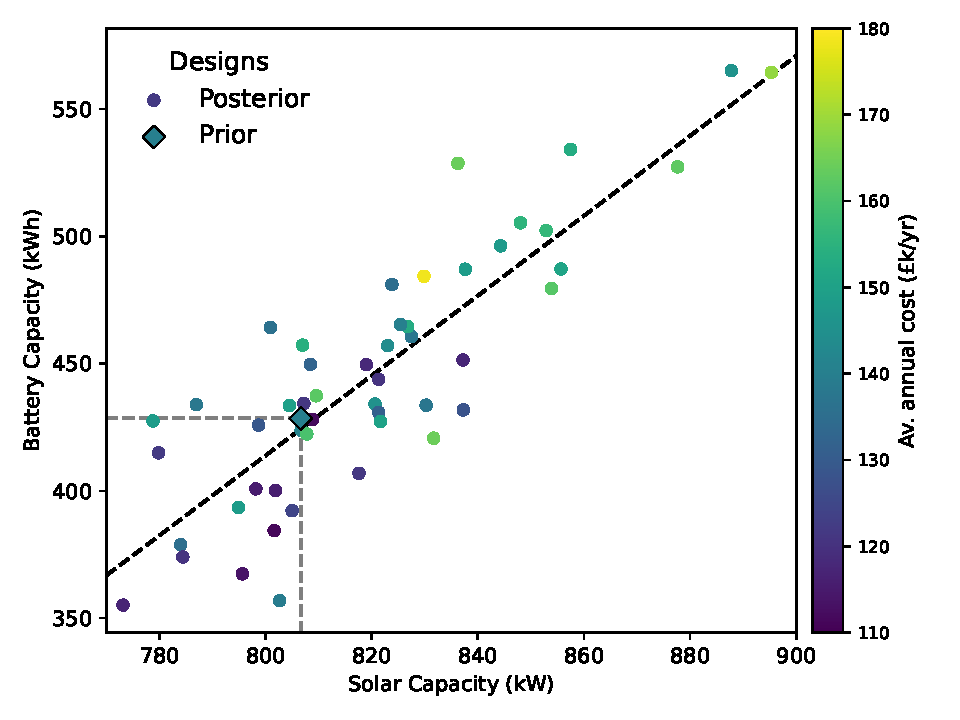
\includegraphics[width=0.75\linewidth]{prior_vs_posterior_designs.pdf}
        \vspace*{-0.25cm}
        \captionof{figure}{Comparison of initial design and designs made with reduced load uncertainty.}
        \label{fig:methodology-example-post-designs-comparison}
    }
    \bigskip

    As we commented last time, getting this information and reducing the load uncertainty leads us to significantly change our design choice, and we can end up making a design decision quite different from the initial choice we'd make (the prior design). Also, the expected cost of system varies substantially ($\pm$25\%) over the possible load measurements we could receive. This seems to suggest that the load uncertainty is having a significant impact on our decision making, as reducing it leads to large changes in both decision and cost.\\

    But ultimately we're not actually interested in the choice we end up making, but how good a job we can do at solving our problem. The average cost of the designs made with reduced load uncertainty is £139.7k/yr. Meaning the \glsxtrshort{evii} is just £0.2k/yr, or 0.2\% of the prior cost. This is around half the \glsxtrshort{evppi} value from \ref{ebox:evppi}. This means even though the practical measurement removes around 75\% of the uncertainty, it's only providing us 50\% of the benefit for decision making.

    From this perspective, reducing load uncertainty in fact isn't particularly important to our decision making. It wouldn't be worth spending much money collecting this data, as the improvement it provides to our design decision is very small.

    However, it does significantly reduce our uncertainty in how much our energy system will cost, which may be beneficial for financial planning and risk management. This is explored in more detail in \Cref{chap:districts}.
\end{ebox}\


\subsection{Information theoretic \glsxtrshort{voi}}

There is also an information theoretic view on \glsxtrshort{voi}. It takes a purely statistical perspective, and defines the utility as the information content or statistical `surprise' of the outcomes\footnote{`Surprise' is a statistical measure of how surprising or unlikely an outcome is. The more unlikely an outcome, the more you learn (the more information you get relative to the prior) by observing it.}. This means that the expected utilities become entropies,
\begin{equation}
    \mathlarger{u(\theta) = -\log p(\theta) \implies \mathbb{E}_{\theta} \lbrace u(\theta) \rbrace = \sum_{\theta} \left( - p(\theta) \log p(\theta) \right) = H(\theta)}
\end{equation}

\noindent
And so the \glsxtrshort{voi} is the mutual information between the uncertainties and the measured data,
\begin{equation}
    \mathlarger{\text{VoI}(e) = \mathbb{E}_{\theta} \lbrace u(\theta) \rbrace - \mathbb{E}_{\theta,z} \big\lbrace \mathbb{E}_{\vartheta} \lbrace u(\vartheta|z) \rbrace \big\rbrace = H(\theta) - H(\theta|z) = I(\theta\,;z)}
\end{equation}
\smallskip

\noindent
As this view of \glsxtrshort{voi} is purely statistical, it doesn't require a decision making model. This is both an advantage and a flaw. It means that we can calculate \glsxtrshort{voi} values for measurements/uncertainty reduction without having to develop a potentially complicated model of how that uncertainty will be used to information decision making. But as a result, we lose a lot of the interpretability of \glsxtrshort{voi}. The units of \glsxtrshort{voi} are now information `bits', and we cannot know how useful that information will be for supporting our decision making, which is ultimately what we care about. This approach is most useful for comparing the uncertainty reduction provided by different measurements in complex systems\footnote{If the system is too simple the likelihood functions of the measurements already tell us what we need to know.}, and looking at the trade-off between the number of measurements made and total uncertainty reduction.\\


\section{Framework extensions} \label{sec:methodology-framework-extensions}

The decisions that need to be made in real-world engineering problems have complexities that cannot be handled by the standard \glsxtrshort{voi} framework that we've seen so far. This section presents two extensions to the framework that allow us to investigate the value of uncertainty reduction to improve decision making in more complex settings.

\subsection{On-Policy \glsxtrlong{voi}} \label{sec:methodology-on-policy-voi}

So far, the \glsxtrshort{voi} calculations have assumed that we have access to an accurate model of the system that we are able to optimise to find the decision/action that provides the highest expected utility, and also tell us that expected utility. However, many practical engineering problems are too complex for an accurate model of the system to be optimised directly. Instead, decisions are made using policies, such as Rule-based Control, Reinforcement Learning, or \glsxtrlong{sp}. These policies either use heuristics to guide their choice of, or search through, actions, or they simplify the system model and/or the statistical representation of the uncertainties\footnote{The most common example of this is the use of Monte Carlo approximations of the expected utility which use only a small number of samples to limit the computational cost of the model, but come at the expense of significant statistical error in the estimate.} and/or the optimisation objective (utility model), to provide an approximate model that is computationally manageable and can be optimised. As a result, a policy may not provide a sufficiently accurate\footnote{Or in some cases even estimate the expected utility at all.} estimate of the expected utility to provide useful \glsxtrshort{voi} values. I.e. the errors in the expected utility estimates may be larger than the \glsxtrshort{voi}, and lead to extremely noisy \glsxtrshort{voi} estimates.\\

To extend the standard \glsxtrshort{voi} framework to allow decision making via policies, an additional step is added to the computations, which estimates the expected utility achieved by the actions selected by the policy using a more accurate model of the system, uncertainties, and utility.

A decision policy is defined as a mapping from a utility function describing a system, $u(a,\theta)$, and a distribution describing the uncertainties in the system, $\pi(\theta)$, to an action,
\begin{equation} \label{eq:policy-defn}
    \mathlarger{\mathcal{P} \left( u(a,\theta),\pi(\theta) \right) \rightarrow \alpha \in \mathcal{A}}
\end{equation}

As the utility function and set of possible actions are constant when we're looking at a given decision problem, we'll simplify the notation and refer to a policy applied to a given decision problem as $\mathcal{P}_u(\pi(\theta))$. The action selected by the policy therefore depends on the uncertainties in the system\footnote{However we don't impose any conditions on how the policy uses the statistical information about the uncertainties, $\pi(\theta)$. The policy could be deterministic. For example it could use only the expected (or maximum likelihood) values of the uncertainties from the distribution. In fact, this is what the \glsxtrlong{evp} does, and so it is a heuristic policy.}.\\

The \glsxtrshort{voi} calculations proceed in the same way as before (compare to Eq. \ref{eq:evii}), but instead of selecting actions using a stochastic optimisation, they are now selected by applying the policy to the relevant distribution of uncertainties, and the expected utility those actions achieve needs to be evaluated using the utility function/model.
\begin{equation} \label{eq:OP-voi}
    \mathlarger{
        \text{EVII}_{\mathcal{P}}(e) =
        \mathbb{E}_{\theta,z} \left\lbrace \mathbb{E}_{\vartheta|z} \left\lbrace u\!\left( \mathcal{P}_u\!\left(\pi (\theta|z)\right)\!,\vartheta \right) \right\rbrace\!\!\right\rbrace
        - \mathbb{E}_{\theta} \left\lbrace u\!\left(\mathcal{P}_u\!\left(\pi (\theta)\right)\!,\theta \right)\!\right\rbrace
    }
\end{equation}
where the $\mathcal{P}$ subscript indicates that this is the value of uncertainty reduction for supporting decisions made using policy $\mathcal{P}$.\\

This framework extension is called `On-Policy \glsxtrlong{voi}', as the decisions are made using a specific policy, and so the benefit of data collection/uncertainty reduction calculated is now dependent on the policy used. This broadens one of the main criticisms of the \glsxtrshort{voi} framework, namely that \glsxtrshort{voi} values do not generalise. This criticism is discussed further in \Cref{sec:methodology-limitations}. However, this does also open up the opportunity to study how different policies benefit from uncertainty reduction, and which are best able to exploit improved statistical information.

The key advantage of On-Policy \glsxtrshort{voi} is that is allows us to study the value of information for complex, practical engineering problems where decision policies have to be used. For instance, problems with high-dimensional actions (i.e. where a large number of decisions must be made simultaneously), or those with tight computational limitations.

\begin{ebox}{Using a decision policy}
    Throughout our example problem we've been using a Stochastic Program, specifically a linear scenario program, to perform our design optimisation and make decisions for us. This \glsxtrshort{sp} uses a simplified model of the energy system, it is linearised and assumes perfect foresight. Also, to keep the computation time manageable, when we solve the posterior decision problems we've only been using 10 samples from the posterior distributions of the uncertainties, leading to quite a noisy estimate of the expected utility.

    So we are actually already using a policy to make our decisions. And there's potentially quite a bit of error in our estimate of the expected utility from both the model and statistical simplification. We could create a more accurate simulator of our building energy system, and apply it to more samples from the posterior distributions to get a more accurate estimate of the expected utilities, and use this to do an On-Policy \glsxtrshort{voi} calculation. However this is a bit too complicated for our simple example.
    You can see On-Policy \glsxtrshort{voi} calculations for a more complex building energy system in \Cref{chap:districts}.
\end{ebox}\


\subsection{\glsxtrlong{voo}} \label{sec:methodology-optionality}

% OG paper with similar idea \citep{merkhofer1977ValueInformationGiven}. \citep{zhang2021ValueInformationAnalysis} also includes this as a framework extension (they call it EVSIA), so it's not new

Standard \glsxtrshort{voi} calculations also assume that when decisions are made with and without data collection/uncertainty reduction, the set of possible actions is the same. However in many practical engineering problems, collecting data leads to a delay\footnote{This delay may form part of the cost of collecting data.} before the decision is taken, and keeping decision options available through this delay is costly, even if those options do not end up being used.\\

We can adapt the \glsxtrshort{voi} framework to study the effect that changing the set of available actions has on decision making as uncertainty is reduced. This is referred to as the \glsxtrlong{voo} (\glsxtrshort{voo}).

If after data collection, the set of available actions is reduced from an initial set, $\mathcal{A}$, to a smaller set, $\mathcal{B} \subset \mathcal{A}$. Then the improvement in decision making that would be achieved by maintaining optionality, and keeping the original set of actions for the decision made with reduced uncertainty, referred to as the \glsxtrlong{evo} (\glsxtrshort{evo}), is given by,

\begin{align}
\begin{split} \label{eq:methodology-voo}
    \mathlarger{\text{EVO}(\mathcal{B},e)} \:
    &\mathlarger{
        = \mathbb{E}_{\theta,z} \left\lbrace \max_{a \in \mathcal{A}} \: \mathbb{E}_{\vartheta|z}\lbrace u(a,\vartheta) \rbrace \!\right\rbrace - \mathbb{E}_{\theta,z} \left\lbrace \max_{a \in \mathcal{B}} \: \mathbb{E}_{\vartheta|z}\lbrace u(a,\vartheta) \rbrace \!\right\rbrace
    }\\[1ex]
    &\mathlarger{
        = \mathbb{E}_{\theta,z} \left\lbrace \max_{a \in \mathcal{A}} \: \mathbb{E}_{\vartheta|z}\lbrace u(a,\vartheta) \rbrace - \max_{a \in \mathcal{B}} \: \mathbb{E}_{\vartheta|z}\lbrace u(a,\vartheta) \rbrace \!\right\rbrace
    }
\end{split}
\end{align}
Notice that the inner term is zero unless we use the optionality and choose an action outside of the reduced set $\mathcal{B}$ when data $z$ is collected. This equation could also be expressed as a difference of \glsxtrshort{voi} values.\\

Similarly to the \glsxtrshort{voi}, the \glsxtrshort{voo} tells us how much better we do on average at solving our problem by maintaining optionality and being able to choose from the full set of actions\footnote{We could also investigate the benefit of increasing the set of actions available to us.} when uncertainty has been reduced. By comparing the benefit optionality provides to decision making to the cost of keeping those options available, we can determine if maintaining optionality is worthwhile.\\

\begin{ebox}{Exploring optionality}
    For the design of our building energy system, we likely have a number of different options for decarbonising the energy usage. For example, instead of installing Li-ion battery storage we could instead install heat pumps, a hot water storage system, or mechanical ventilation with heat recovery (MVHR). We will likely go through an initial design phase and choose one of these approaches. After this, we'll do a more detailed design of the system, and gather some data about the building to help with this, for instance the historic electrical \& heating loads and more precise data on the specs of our chosen system. However, the best decarbonisation approach depends on how much electricity and heat the building will use, and how our energy system performs. So after we've reduce these uncertainties we may find out a different approach than the one we initially chose would actually be better. But we're committed now.

    We could perform a \glsxtrshort{voo} calculation to see how much we could save by doing a preliminary design for all configurations of the energy system, gathering the building load data and tech specs from the equipment manufacturers, and then choosing the best approach after the uncertainties have been reduced. With this we could determine whether the extra time and effort required to provide this optionality is worthwhile, or if our initial design choice is good enough.

    Again, doing this calculation is a bit complicated for our simple example. But a \glsxtrshort{voo} calculation is performed in the context of energy storage technology selection for an industrial scale energy park in \Cref{chap:parks}.
\end{ebox}\


%********************************** VoI discussions **************************************
\section{Limitations of framework} \label{sec:methodology-limitations}

% lack of generalisation guarantees (though this applied to lots of engineering analyses, VoI can be particularly sensitive, discuss why?) - overcome with sensitivity analysis (but even more expensive)
% models are necessarily limited, so some judgement is needed at to whether it's good enough; particularly difficult as adding in new uncertainties (even non-reducible) can change the VoI, so model completeness is a concern
% computational cost, we need to do optimisation based design potentially hundreds of times - limits model complexity, accuracy, and scope
% it also requires to actually be able to come up with a decision model of the system - can only be used for automated decision making with a single objective (no multi-objective), this modelling is hard, and we can't account for more holistic factors in decision making
% only VoI contained within model is accounted for, there may be other uses for the data collected that aren't captured in the decision model, e.g. unknown future uses, or retro-active decisions - though in this case it gives us a much more defined value to guess (gap between VoI and collection cost)
% assumption of risk neutrality - overcome with risk aversion utility functions (e.g. CVaR in Chap:districts)

The key limitation of \glsxtrshort{voi} analysis is that the \glsxtrshort{voi} values calculated are only valid for the particular system model, statistical model, decision objective, and policy used. The framework does not provide any guarantees that the conclusions about which and how much data should be collected will generalise to other systems, or even with changes to the current model and its assumptions. So care needs to be taken when interpreting and communicating the insights provided by the \glsxtrshort{voi}, being clear that the conclusions only apply to how data collection is used to support the specific decision made within the assumptions and limitations of the model. Of course this is a very common limitation of engineering analyses, particularly optimisation modelling. Generalisation guarantees are difficult to provide, and at some point judgement is required as to whether a model is a good enough representation of the practical engineering problem. However, \glsxtrshort{voi} can be particularly sensitive to the model setup. This is because \glsxtrshort{voi} values depend on the utility values at the optima, which can move significantly and unexpectedly as the model changes. Seemingly innocuous changes to the model can cause large changes in \glsxtrshort{voi}, for example if they lead to a dominant action which causes the \glsxtrshort{voi} to drop to zero. Adding new uncertainties into the model can also affect the \glsxtrshort{voi}, even if those uncertainties are not measured and reduced.

This generalisation limitation can be overcome by performing sensitivity analyses to test whether the conclusions drawn remain valid as the model setup and assumptions change. However, this is very computationally expensive, and it's not possible to test all model variations that could be relevant. Particularly as performing \glsxtrshort{voi} calculations is already highly computationally expensive.\\

The second main limitation is the computational cost of calculating the \glsxtrshort{voi}. In \glsxtrshort{voi} analysis we are testing how the decision optimisation changes as different data values are observed. Outside of very simple analytic cases, this requires us to sample possible data values and repeat the decision optimisation a large number of times to get a good \glsxtrshort{mc} estimate of how well we can do on average when making decisions with data. So computing a single \glsxtrshort{voi} value requires likely hundreds of optimisations to be performed. For practically useful problems, these optimisations are themselves computationally expensive. This means that either expensive compute resources\footnote{The optimisations needed for \glsxtrshort{voi} calculations are embarrassingly parallel. So calculations can be performed quickly if enough compute is available.} are needed, the scope of problems considered needs to be limited, or significant simplifications need to be made to the model, which can affect the accuracy of the results. For the \glsxtrshort{voi} calculations in Chapters \ref{chap:districts} \& \ref{chap:parks}, a supercomputer\footnote{The experiments were run using the Cambridge Service for Data Driven Discovery (CSD3, \url{www.csd3.cam.ac.uk}).} was needed to run the experiments in an achievable time.

To be able to perform the decision optimisations, we also need to be able to develop a decision-making model of the engineering system, be that a system model that can be optimised or a suitable decision policy. For complex, real-world engineering systems this modelling can be extremely challenging and require significant domain expertise. The \glsxtrshort{voi} framework also requires that we describe outcomes with a single utility value. This means it is not compatible with multi-objective decision making and cannot account for subjective factors of decision making that often occur in engineering design. The framework is most suited to automated or model-based decision making.\\

We collect data for many reasons, and data has many uses. However, \glsxtrshort{voi} calculations only quantify the value of data collection to support the specific decision studied. So if that same data is useful for other purposes not captured by the model, this extra value will be missed by the calculated \glsxtrshort{voi}. It's difficult, for example, to describe how useful having a historic record of some measurement of a system might be to inform future decision making, such as maintenance. However, having the \glsxtrshort{voi} value helps us make these finer judgements about whether data is worthwhile collecting. With knowledge of the value of that data for supporting the known and modellable decisions, and the cost of collecting the data, we only need to judge whether we think the extra value we might get from the data justifies that difference between the known benefit and the cost. And it may turn out that the data is already worth collecting on the basis of the known decisions.

Finally, the standard \glsxtrshort{voi} framework assumes that decisions are made in a risk-neutral way. This comes from the optimisation objective being the expected/average utility. However many real-world decision makers are risk averse, particularly those making large financial investments to decarbonise energy. The framework can easily be adapted to account for risk aversion in decision making by including it the decision objective. This allows us to study how uncertainty reduction affects decision risk, as is done in \Cref{chap:parks}.\\

\begin{ebox}{Understanding and overcoming our limitations}
    % What are the limitations in our example? And what could we do to overcome them?
    In our example problem, we found that collecting electricity meter data to reduce the uncertainty in the building load provided little benefit for improving our design decision of sizing the solar-battery system. But the calculations we've done only apply to the specific building energy model we've used, the probabilistic models of the uncertainties, and our decision objective. All of these contain simplifications and assumptions which might not be the same for other buildings. So to make a more general statement about the value of energy usage data for supporting building energy system design, we'd need to see whether our conclusion stays the same when we adapt our model to the properties of other buildings. For example, domestic buildings will have different load distributions and energy sale prices.

    To make our example computationally achievable, we've had to make some significant simplifications to the building energy model. We've linearised the physics and assumed perfect foresight. Potentially if we used a more realistic model we might get quite different cost values, which could alter the \glsxtrshort{voi}. There are also some uncertainties we haven't included in the model, for example uncertainty in the cost of solar panels, which might also affect the \glsxtrshort{voi}.

    To keep the computation time down, we had to use quite a small number of samples from the posterior distributions. So there might be quite significant statistical error in our estimate of the \glsxtrshort{voi} values. To test this, we should perform some more samples and see whether the \glsxtrshort{voi} values change significantly, or whether the estimates have already converged.
\end{ebox}\


% \section{Computing \glsxtrshort{voi} in practice} \label{sec:methodology-considerations}

% \subsection{Modelling the problem}

% The hardest part of VoI is modelling the problem. Here are the components you need ...

% \subsection{Computational workflow}

% Nice flow diagram of generalised workflow explaining each step - adapt workflow from BD-VOI methodology section - link to influence diagram

% \subsection{Improving computational efficiency}

% The main bottleneck in VoI calculations is the computational cost (getting it low enough to actually get a decent statistical estimate of the VoI), so here are some considerations to improve the efficiency of the calculations

% Probably keep each subsection brief and just mention the possible options to explore

% \subsubsection{Modelling choices} \label{sec:methodology-modelling-choices}

% Both for probabilistic models and for decision models

% Discretisation, linearisation/convexification, analytic approximations \citep{wilson2015PracticalGuideValue} (much stricter modelling assumptions), surrogate models (e.g. GPs - sort of numerical/analytic hybrid), etc. - trade-off of speed and accuracy

% \subsubsection{Accelerating computation}

% Fundamental parallelisability, ability to split up statistical and optimisation parts, etc.

% \subsubsection{Statistical techniques}

% Importance sampling?, scenario reduction methods, etc.; trying to get more accurate estimates with fewer samples

% \subsubsection{Understanding accuracy}

% Discuss open problem of VoI accuracy estimation


\newpage
%********************************** Model definition appendix  **************************************
\begin{subappendices}

\section{Simple building energy system model for example problem} \label{app:example-problem-formulation}

% Intro and explain simple energy system model, why we use a Linear Program, how it works in simulation and design mode, etc.

For our example problem of designing (specifically sizing) a solar-battery system for a commercial building, we'll consider a simplified model of the building energy system. This system has four key components: the building electrical load which needs to be met (we'll assume the heating is electrified), the solar panels which generate electricity, the battery storage system which can store and release electricity, and the grid from which we can buy and sell electricity. Fig. \ref{fig:example-system-diagram} illustrates the energy flows in this energy system model.

\begin{figure}[h]
    \centering
    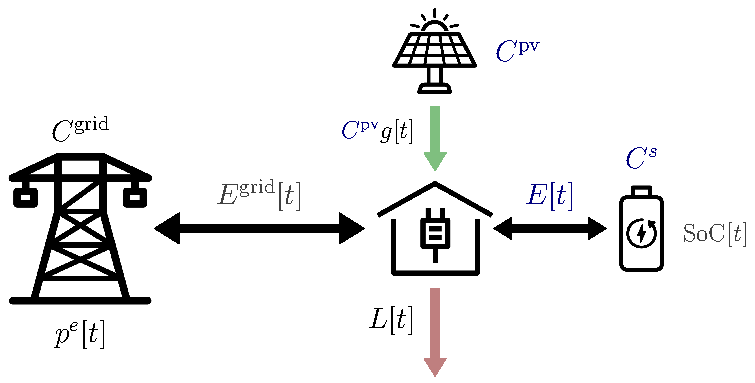
\includegraphics[width=0.75\linewidth]{System Diagram/sys-diagram.pdf}
    \caption{Illustration of energy flows in example building energy system.} \label{fig:example-system-diagram}
\end{figure}

\subsection{Energy model}

We can create a linear model of the behaviour of this energy system by assuming that the only physics we need to satisfy is the conservation of energy, and that the properties of the solar panels and battery storage system (e.g. efficiency, power limits, etc.) are fixed/constant. We will treat the building load, generation potential of the solar panels, and price of grid electricity as exogenous, but potentially uncertain.

Our goal is to design the system to minimise the total cost of meeting the building's energy demands. This is made up of the cost of installing the solar panels and battery storage, the cost of buying electricity from the grid, and the revenue from selling excess electricity back to the grid. To reduce computation, we'll simulate one year of operation of the system and compute the annualised total cost. It's assumed that when we sell electricity back to the grid, we receive some fraction of the market price we would buy at, and that there is a constraint on the maximum power that can be drawn from the grid, i.e. a grid connection capacity.

This linearised model of the energy system can be described using a Linear Program (\glsxtrshort{lp}). This is given by Eq. \ref{eq:example-lp}, with the parameters of described in \Cref{tab:example-problem-params}. A software implementation of this \glsxtrshort{lp} is available \href{https://github.com/mal84emma/VoI-Tutorial/blob/main/models/energy_model.py}{here}.

The model can be run either in simulation or design mode. In simulation mode, capacities for the solar and storage are specified, and the operation of the system (scheduling of the battery storage) is optimised, meaning the model returns the annualised total cost of the specified design if it were operated optimally. In design mode, the capacities of the solar and storage are included as decision variables in the optimisation, meaning the model simultaneously optimises the operation and sizing of the system, returning the lowest possible annualised total cost and the system design that achieves it.

For the example experiments we will use historic building load monitoring data from a university building in Cambridge\footnote{Specifically, we use the load data from Building 0 in the dataset from \Cref{chap:districts} for this simple example problem.} , as well as solar generation and electricity pricing data from the area. This is the same data that is used for the investigation in \Cref{chap:districts}. In fact, \Cref{chap:districts} is just a more complex version of this example problem. The other parameter values used in the experiments are given in \Cref{tab:example-problem-param-values}.\\

\renewcommand{\arraystretch}{1}
\begin{subequations} \label{eq:example-problem-formulation}
    \begin{align}
        \addtocounter{equation}{-1}
        \text{min} & \qquad p^{\textrm{pv}} C^{\textrm{pv}} + \mathlarger{\mathlarger{\sum}}_m \: \rho_m \left( p^s_m C^s + \mathlarger{\sum}_t \: p^e[t] \left( \left[E^{\text{grid}}_m[t]\right]^+ + \kappa \left[E^{\text{grid}}_m[t]\right]^- \right) \right)
        \label{eq:example-lp} \\[\eqnskip]%%
        %%
        \text{over} & \qquad C^{\textrm{pv}},\, C^s,\, E_m[t],\, \textrm{SoC}_m[t{+}1] \quad \forall \: m,\, t \tag*{} \\[\eqnskip]%%
        %%
        \text{subject to} & \qquad \textrm{SoC}_m[t{+}1] = \textrm{SoC}_m[t] + \sqrt{\eta_m} \left[E_m[t]\right]^{+} - 1/\sqrt{\eta_m} \left[\, E_m[t] \right]^{-} \label{eq:example-dynamics-constraint} \\[\smalleqnskip]
        & \qquad -P^{\textrm{max}} \Delta t \leq E_{i,m}[t] \leq P^{\textrm{max}} \Delta t \label{eq:example-power-constraint} \\[\smalleqnskip]
        & \qquad (1{-}\nu)\, C^s \leq \textrm{SoC}_m[t{+}1] \leq C^s \label{eq:example-energy-constraint} \\[\smalleqnskip]
        & \qquad P^{\textrm{max}} = \delta C^s \label{eq:example-power-capacity} \\[\smalleqnskip]
        & \qquad \textrm{SoC}_m[0] = \textrm{SoC}^0 C^s \label{eq:example-initial-conditions} \\[\smalleqnskip]
        & \qquad E^{\text{grid}}_m[t] = L_{m}[t] - C^{\textrm{pv}} g_m^{\textrm{pv}}[t] + E_m[t] \label{eq:example-grid-variable} \\[\smalleqnskip]
        & \qquad E^{\text{grid}}_m[t] \leq C^{\text{grid}} \Delta t \label{eq:example-grid-cap} \\[\smalleqnskip]
        %& \qquad C^{\text{pv}} \leq C^{\text{pv}}_{\max} \\[\smalleqnskip]
        %& \qquad p^{\textrm{pv}} C^{\textrm{pv}} + p^{\textrm{w}} C^{\textrm{w}} + \mathlarger{\sum}_i \: p^s_{i,m} C^s_i \leq B^{\text{cap}} \label{eq:budget-cap} \\[\smalleqnskip]
        %%
        \text{for all} & \qquad m \in [0,M{-}1], \: t \in [0,T{-}1] \tag*{}
        \end{align}
\end{subequations}

\begin{table}[hp]
    \centering
    \renewcommand{\arraystretch}{1.2}
    \begin{tabularx}{\linewidth}{ccX} \toprule \toprule
        Parameter & Units & \multicolumn{1}{>{\centering\arraybackslash}c}{Description} \\
        \midrule \midrule
        \multicolumn{3}{>{\centering\arraybackslash}l}{\small \quad Decision variables} \\
        $C^{\textrm{pv}}$ & kWp & Installed solar PV capacity \\
        $C^s$ & kWh & Installed energy capacity of battery storage \\
        $E_m[t]$ & kWh & Energy flow \textit{into} battery storage at time $t$ in scenario $m$ \\
        $\textrm{SoC}_m[t]$ & kWh & State-of-charge of battery storage at time $t$ in scenario $m$ \\
        \midrule
        \multicolumn{3}{>{\centering\arraybackslash}l}{\small \quad Derived variables} \\
        $E^{\text{grid}}_m[t]$ & kWh & Net energy \textit{drawn from} electricity grid at time $t$ in scenario $m$ \\
        $P^{\textrm{max}}$ & kW & Power capacity of battery storage \\
        \midrule
        \multicolumn{3}{>{\centering\arraybackslash}l}{\small \quad Sampled parameters} \\
        $\rho_m$ & -- & Probability of scenario $m$ \\
        $L_m[t]$ & kWh & Building electrical load at time $t$ in scenario $m$ \\
        $g_m^{\text{pv}}[t]$ & kWh/kWp & Solar PV power generation potential at time $t$ in scenario $m$ \\
        $\eta_m$ & -- & Round-trip efficiency of battery storage in scenario $m$ \\
        $p^s_m$ & £/kWh/yr & Annualized capacity cost\textsuperscript{\textdagger} of battery storage in scenario $m$ \\
        \midrule
        \multicolumn{3}{>{\centering\arraybackslash}l}{\small \quad Known parameters} \\
        $\Delta t$ & hrs & Time step of simulation data \\
        $\delta$ & kW/kWh & \makecell[l]{Discharge ratio of battery storage\\(power capacity/energy capacity)} \\
        $\nu$ & -- & Depth-of-discharge of battery storage \\
        $\textrm{SoC}^0$ & -- &  Initial state-of-charge of battery storage (fraction of capacity) \\
        $C^{\text{grid}}$ & kW & Grid connection capacity \\
        $p^{\text{pv}}$ & £/kWp/yr & Annualized capacity cost\textsuperscript{\textdagger} of solar PV \\
        $p^e[t]$ & £/kWh & Price of grid electricity at time $t$ \\
        $\kappa$ & -- & Electricity sell price as fraction of buy price \\
        %$p^c$ & £/kgCO$_2$ & Nominal carbon price \\
        %$c[t]$ & kgCO$_2$/kWh & Carbon intensity of grid electricity at time $t$ \\
        %$C^{\text{pv}}_{\max}$ & kWp & Solar capacity limit \\
        %$B^{\text{cap}}$ & £/yr & Capital budget constraint \\
        \midrule
        \multicolumn{3}{>{\centering\arraybackslash}l}{\small \quad Indices} \\
        %$i$ & -- & Storage technology \\
        $t$ & -- & Time step in modelled operation \\
        $m$ & -- & Scenario number \\
        \bottomrule \bottomrule
    \end{tabularx}
    \smallskip
    \caption{Description of variables \& parameters of Stochastic Program, Eq. \ref{eq:example-lp}.} \label{tab:example-problem-params}
    \footnotesize{\textsuperscript{\textdagger}\,Capital cost per energy/power capacity per year of lifetime}
\end{table}

\begin{table}[h]
    \centering
    \renewcommand{\arraystretch}{1}
    \renewcommand\cellset{\renewcommand\arraystretch{0.33}%
        \setlength\extrarowheight{0pt}}
    \begin{tabularx}{\linewidth}{lccX} \toprule \toprule
        \multicolumn{1}{>{\centering\arraybackslash}c}{Parameter} & Units & Value & \multicolumn{1}{>{\centering\arraybackslash}c}{References} \\
        \midrule \midrule
        Simulation duration, $T$ & Hours & 8760 & \\
        Simulation time step, $\Delta t$ & Hours & 1 & \\
        Discharge ratio, $\delta$ & kWp/kWh & 2 & \citep{kebede2022ComprehensiveReviewStationary} \\
        Depth-of-discharge, $\nu$ & -- & 0.9 & \citep{irena2017ElectricityStorageRenewables} \\
        Initial state-of-charge, $\text{SoC}^0$ & -- & 0.75 & \\
        Grid capacity, $C^{\text{grid}}$ & kW & 500 & \\
        Annualised cost of solar PV & £/kWp/yr & 75 & \citep{ramasamy2023SolarPhotovoltaicSystem} \\
        Fractional sell price, $\kappa$ & -- & 0.5 & \\
        %Solar capacity limit, $C^{\text{pv}}_{\max}$ & MW & 500 & \\
        \midrule
        \multicolumn{4}{>{\centering\arraybackslash}l}{\small\it Default values of uncertain parameters} \\
        Solar year & -- & 2017 & \\
        Load year & -- & 2017 & \\
        Average building load & kW & 100 & \\
        Battery efficiency, $\eta$ & -- & 0.95 & \\
        Battery cost, $p^s$ & £/kWh/yr & 70 & \citep{forbeshome2024HowMuchDoes} \\
        \bottomrule \bottomrule
    \end{tabularx}
    \smallskip
    \caption{Parameter values for example building energy system model.}
    \label{tab:example-problem-param-values}
\end{table}

\newpage
\subsection{Probabilistic model of uncertainties} \label{app:example-problem-uncertainties}

In our example we'll look at uncertainties in the building load, solar generation, and battery storage. Where uncertainties in these factors are considered, we'll use the probabilistic models given in \Cref{tab:example-problem-distributions}, otherwise we'll treat them as fixed and use the values given in \Cref{tab:example-problem-param-values}.

The uncertainty in the building load is represented using two parameters: the load year which represents the uncertainty in the shape and timing of the load profile, and the average building load. Years of load data are sampled uniformly from the available dataset.\\

\begin{table}[h]
    \centering
    \renewcommand{\arraystretch}{1.25}
    \begin{tabularx}{0.875\linewidth}{l@{\hskip 5mm}|c@{\hskip 5mm}c@{\hskip 5mm}c} \toprule \toprule
        \multicolumn{1}{>{\centering\arraybackslash}c|}{Parameter} & Distribution & Parameters & Units \\
        \midrule \midrule
        Solar year & \multirow{2}{*}{Discrete uniform} & $\lbrace 2012,\dots,2017 \rbrace$ & -- \\
        Load year & & $\lbrace 2012,\dots,2017 \rbrace$ & -- \\
        Average building load & \multirow{3}{*}{\makecell{Truncated Normal\\{\small (cut-off at $\pm2\sigma$)}}} & $\mu{=}100$, $\sigma{=}10$ & MW \\
        Battery efficiency, $\eta$ & & $\mu{=}0.95$, $\sigma{=}0.05$ & -- \\
        Battery cost, $p^s$ & & $\mu{=}70$, $\sigma{=}5$ & £/kWh/yr \\
        \bottomrule \bottomrule
    \end{tabularx}
    \smallskip
    \caption{Distributions of uncertainties.}
    \label{tab:example-problem-distributions}
\end{table}


\subsection{A brief tirade on constraints in statistical optimisation} \label{app:methodology-constraints-tirade}

The mathematics of optimisation do not sit very comfortably with a probabilistic view of the world. This is especially true when it comes to constraints. Mathematical constraints are written as strict laws that the problem must adhere to. But when we come to solve optimisation problems numerically, Lagrangian optimisation treats these constraints in the same way as the objective \citep{boyd2004ConvexOptimization}, and allows us to violate them, though our solvers try not to. In the real world there are some strict constraints, we have to obey the laws of physics. But often we impose practical engineering constraints on our system that are somewhat artificial.

The problem comes when we try to model uncertainties in our system that interact with these constraints. If we don't account for the full value range of the uncertainties it's possible that we will end up making decisions that will violate the constraints in some possible realisations. But, if we try to make decisions that will satisfy the constraints in every possible outcome we'll end up being far too conservative. The issue is that in our optimisation we can't differentiate between the hard constraints we \textit{have} to obey, and the softer constraints where there is potentially some flexibility.

For instance, in our example problem the deterministic \glsxtrshort{lp} chooses a system design that is infeasible when we start accounting for uncertainty in the solar generation. This is because the design puts in a large solar generation capacity, and in years where the sun is more intense, the solar power ends up exceeding the grid connection capacity. From a mathematical perspective it's difficult to know what to do in this case. Our optimisation simply fails. In reality, there is likely to just be some cost associated with exceeding the grid connection capacity, either a charge from the grid operator \citep{frontiereconomics2022NetworkTariffsEnergy} or a cost associated with having to disconnect the solar panels and causing some damage to the system.

Because we have no clear way of dealing with infeasibility and failed optimisations, we instead need to model our energy systems in such a way that our uncertainties cannot lead to violation of the constraints. Where we have soft constraints, we should instead model the costs associated with violating them and include these in the objective, as is done for grid connection capacity in \Cref{chap:districts}. Ultimately we need to consider how our system will actually behave when things go wrong, and account for the associated costs in our decision making. A classic example of this in the energy systems literature is constraining energy systems to have some specified loss-of-load probability. This constraint is quite arbitrary, and is very hard to guarantee. Instead we should be concerned with the cost of not satisfying the load, as we can then account for this cost trade-off when we design the energy system.

\end{subappendices}